\documentclass[a4paper,crop=false]{standalone}
% \usepackage{amsmath}
% \usepackage{amssymb}
% \usepackage{fullpage}
% \usepackage[compat=1.1.0]{tikz-feynman}
% \usepackage{wrapfig}
% \usepackage{hyperref}
% \usepackage{graphicx,subcaption,caption}
\begin{document}
        For the first valley, at one loop, we have the diagram

        \begin{wrapfigure}{r}{0.3\textwidth}
            % \centering
            \begin{tikzpicture}
            %     \begin{feynman}
            %         \vertex (b);
            %         \vertex [left=of b] (a);
            %         \vertex [right=of b] (c);

            %         \diagram*{
            %             (a) -- (b)[dot] --[out=135,in=45,loop,min distance = 3cm] (b) -- (c),
            %         };
            %     \end{feynman}
            \feynmandiagram [horizontal=a to b, layered layout] {
                a -- [fermion,edge label'=\(k_1\)] b [dot] -- [fermion, out=135, in=45, loop, min distance=3cm,edge label'=\(k\)] b -- [fermion,,edge label'=\(k_4\)]c,
            };

            \end{tikzpicture}
            \caption{one loop diagram for two point function}
            \label{fig:tadpolefromV1}
        \end{wrapfigure}

        This diagram \ref{fig:tadpolefromV1} evaluates to
        \begin{equation}\label{eqn:bubble}
            V_1\int^{\infty}_{-\infty} \frac{d\omega}{2\pi}\int_{\frac{\Lambda}{s}<|k|<\Lambda} \frac{d^2k}{(2\pi)^2}G^{(0)}_1(i\omega,k )
        \end{equation}
        We will first evaluate the $\omega$ integral. The poles are at $\pm iv_F|k|$. We can close the loop on either side to get contribution from only one of the pole. For example lets close the loop on the upper half complexplane to get.
        \begin{equation}
            V_1\int_{\frac{\Lambda}{s}<|k|<\Lambda} \frac{d^2k}{(2\pi)^2} \frac{v_F |k| + v_F\sigma . k}{2v_F |k|} = V_1 \int_{\frac{\Lambda}{s}<|k|<\Lambda} \frac{d^2k}{(2\pi)^2}\frac{1}{2}\left( 1 + \frac{\sigma . k}{|k|} \right)
        \end{equation}
        The $\sigma . k$ part vanishes as it is an odd function of k. The other part gives
        \begin{equation}
            V_1 \int^{\Lambda}_{\frac{\Lambda}{s}} \frac{2\pi k dk}{(2\pi)^2}\frac{1}{2} = \frac{V_1\Lambda^2}{8\pi}\left( 1 - \frac{1}{s^2} \right)
        \end{equation}
        \begin{mybox}{Note}
            This introduces a term in the Hamiltonian of the form $\Psi^{\dagger}_{1,q} \left(\frac{V_1\Lambda^2}{8\pi}\left( 1 - \frac{1}{s^2} \right) \right)\Psi_{1,q}$. It looks like a chemical potential term which can be tuned to remove the term.
        \end{mybox}

\end{document}